\Section{Сетевой уровень TCP/IP}{Лекции 2-3}{Игорь Смирнов}

Протоколы:
\begin{itemize}
    \item IP~--- основной протокол архитектуры TCP/IP
    \item ICMP~--- протокол управляющих сообщений
    \item IGMP~--- протокол работы с группами
    \item ARP~--- протокол разрешения адресов~--- связь между собой адресов канального и сетевого уровней
    \item Протоколы маршрутизации
\end{itemize}

\Subsection{Протокол IP}

{\bf IP}~--- Internet Protocol

Стандарт RFC 791, 1981 год

Текущая действующая версия~--- 4 (IPv4)

Состоит из заголовка и тела

Суммарная длина до 64 Кбайт

Структура IP-пакета:

\begin{figure}[H]
  \centering
  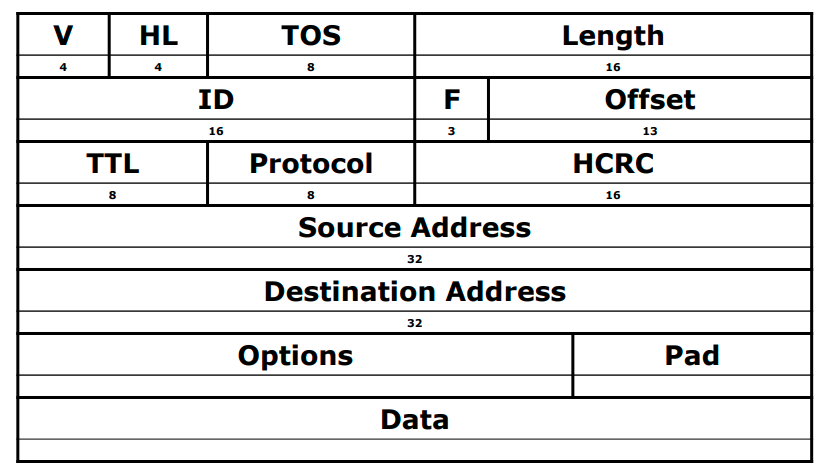
\includegraphics[width=15cm]{images/02/01}
\end{figure}

Ширина картинки~--- 32 разряда. Под каждым полем подписано, сколько разрядов оно занимает.

\begin{itemize}
    \item V~--- версия протокола
    \item HL~--- длина заголовка в 32-разрядных словах
    \item TOS~--- пожелания к процедуре обслуживания данного пакета
    \item Length~--- длина пакета в байтах
    \item ID~--- идентификатор (для фрагментации)
    \item F~--- флаги (для фрагментации)
    \item Offset~--- смещение (для фрагментации)
    \item TTL~--- время жизни
    \item Protocol~--- вложенный протокол (в данных)
    \item HCRC~--- контрольная сумма (по заголовку)
    \item Source Address~--- адрес отправителя
    \item Destination Address~--- адрес получателя
    \item Options~--- если пакет нестандартный и требует каких-то опций, можем их включить
    \item Pad~--- заполнитель, если опции не кратны 32 разрядам
    \item Data~--- данные
\end{itemize}

\Subsubsection{Поля заголовка пакета IP}

\begin{itemize}
    \item V~--- версия протокола (4)
    \item HL~--- длина заголовка в 32-разрядных словах (от 5 до 15). По дефолту 5, а эти 10 слов~--- на опции
    \item Length~--- длина пакета в байтах
    \item TTL~--- время жизни. Имело разный смысл. Изначально записывали значение <<время жизни пакета в секундах>> и маршрутизаторы отнимали из него время своей обработки. Сейчас это неактуально. Теперь каждый промежуточный маршрутизатор отнимает единицу. Если маршрутизатор получает 0, он удаляет пакет и посылает обратно ICMP сообщение. Время жизни нужно ограничивать, чтобы не зациклиться (мало ли где-то в сети есть петля маршрутизации). Утверждается, что между любыми узлами в сети интернет не более 29 промежуточных. То есть можно ставить 30.
    \item HCRC~--- контрольная сумма (по заголовку). Считается циклическим полиномом, по которому можно определить, не произошло ли искажения при передаче.
    \item Source Address~--- адрес отправителя
    \item Destination Address~--- адрес получателя
    \item Data~--- данные (тело пакета)
\end{itemize}

А где же записывается маска подсети? Она нужна только для процедуры маршрутизации, чтобы определить, каким путём посылать пакет. Самому пакету маски не нужны. 

\begin{itemize}
    \item Protocol~--- идентификатор вложенного протокола. Список идентификаторов лежит в RFC 1700. В операционных системах есть файл, который содержит код протокола ({\tt /etc/protocols}, {\tt \%systemroot\%$\backslash$system32$\backslash$drivers$\backslash$etc$\backslash$protocol})\\
    Основные протоколы:
    \begin{itemize}
        \item 1~--- ICMP
        \item 2~--- IGMP
        \item 4~--- IP4
        \item 6~--- TCP
        \item 17~--- UDP
        \item 89~--- OSPF
    \end{itemize}
    \item TOS~--- тип сервиса. Пожелания относительно способа доставки. В общем случае, пожелания могут быть проигнорированы. Но внутри своей сети можем запилить.\\
    \begin{figure}[H]
        \centering
        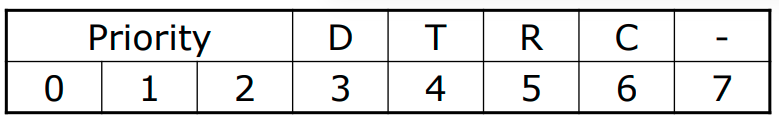
\includegraphics[width=15cm]{images/02/02}
    \end{figure}
    \begin{itemize}
        \item Приоритет (первые 3 разряда). Можно сделать очередь с приоритетом обработки пакетов (внутри своей сети).\\
        0~--- нормальный приоритет\\
        1~--- приоритетный\\
        2~--- немедленный\\
        3~--- мгновенный\\
        4~--- срочный\\
        5~--- критический\\
        6~--- межсетевое управление\\ 
        7~--- сетевое управление\\

        В жизни используются только 0, 1, 6, 7. Даже среди них 99\%~--- приоритет 0

        \item D (delay)~--- требуется минимальная задержка
        \item T (throughput)~--- требуется максимальная пропускная способность
        \item R (reliability)~--- требуется максимальная надёжность
        \item C (cost)~--- требуется минимальная стоимость
    \end{itemize}

    При этом одновременно может быть установлено 1 или 0 флагов.

    Для классических протоколов эти флаги предопределены.

    \begin{figure}[H]
        \centering
        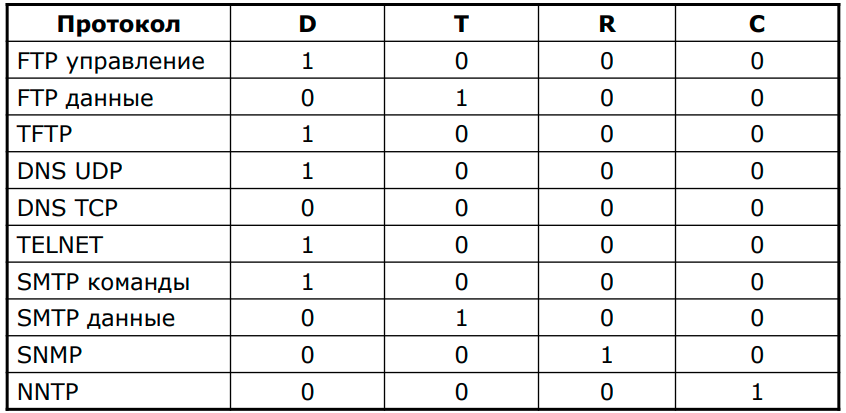
\includegraphics[width=15cm]{images/02/03}
    \end{figure}
\end{itemize}

\Subsubsection{Фрагментация пакетов} 

Напомним, что фрагментация поузловая.

\begin{itemize}
    \item Id~--- идентификатор, одинаковый у всех фрагментов. При передаче IP пакета это поле формируется псевдослучайно
    \item Offset~--- смещение фрагмента относительно начала пакета в 8-ми байтовых словах
    \item F~--- флаги
    \begin{itemize}
        \item 0~--- зарезервировано
        \item 1~--- флаг разрешения фрагментации. Если не установлен, маршрутизатор не имеет права фрагментировать данный пакет. А если она требуется, то пакет уничтожается, а обратно посылается ICMP пакет с ошибкой.
        \item 2~--- признак последнего фрагмента (внезапно, 0, если это последний фрагмент и 1 иначе)
    \end{itemize}

    Благодаря смещению правильно складываем куски в буфере, благодаря флагу последнего пакета понимаем, что все фрагменты пришли.

    На принимающей стороне есть таймер фрагментации, и если за это время все фрагменты не пришли, посылается ICMP сообщение.
\end{itemize}

\Subsubsection{Опции протокола IP}

Идёт прямо перед данными, может быть переменной длины. Может вообще не быть.

Это необязательные опции, используются только в служебных целях.

Формат опций:

\begin{figure}[H]
  \centering
  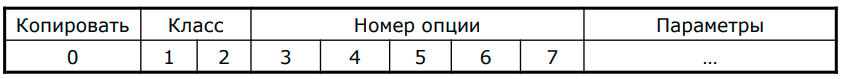
\includegraphics[width=15cm]{images/02/04}
\end{figure}

\begin{itemize}
    \item Флаг копирования~--- 1, если нужно копировать опции во все фрагменты пакета. Если 0, то только в первом фрагменте
    \item Класс опции
    \begin{itemize}
        \item 0~--- управление дейтаграммами или сетью
        \item 1~--- зарезервировано
        \item 2~--- отладка сети
        \item 3~--- зарезервировано
    \end{itemize}
    \item Номер опции~--- номер внутри класса
\end{itemize}

Основные опции:

\begin{figure}[H]
  \centering
  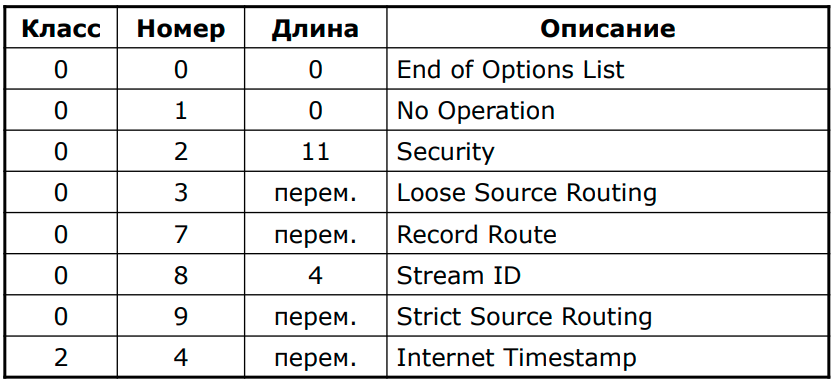
\includegraphics[width=15cm]{images/02/05}
\end{figure}
\begin{itemize}
    \item End of Option List~--- конец списка опций. Говорит, что это последняя опция в пакете. Нужна, если граница опций не совпадает с границей заголовка IP (когда есть паддинг). Занимает 1 байт.
    \item No operation~--- нет операции. Вспомогательная, для выравнивания границы опций, занимает 1 байт
    \item Stream ID~--- идентификатор потока. Например, хотим маршрутизировать видеотрафик. Всем пакетам одного потока присваивается одна метка потока. Понимаем, как маршрутизировать первый из них, а потом остальные маршрутизируем так же. Должна копироваться при фрагментации. Занимает 4 байта: 1 байт на заголовок, 1 байт на длину, 2 байта на идентификатор потока.
    \item Strict Source Route~--- строгая маршрутизация от источника (предопределённая маршрутизация). Пакет имеет право проходить только по адресам, указанным при отправке от источника и строго в указанном порядке.
    \begin{itemize}
        \item Заголовок
        \item Максимальная длина в байтах
        \item Указатель (на каком мы сейчас маршрутизаторе)~--- смещение в байтах от начала опции
        \item Список адресов.
    \end{itemize}
    Максимум можем указать 9 маршрутизаторов (так как есть ограничение на размер опций).
    \item Loose Source Route~--- нестрогая маршрутизация от источника. Содержит адреса маршрутизаторов, через которые должен пройти пакет. Формат такой же, как и раньше. Отличие в том, что мы снова обязаны пройти через все адреса, но при этом могут быть какие-то промежуточные.

    Обе эти опции используются только для отладки.

    \item Record Route~--- запись маршрута. Используется в ping. В traceroute используется более хитрая схема.

    Есть несколько полей. Каждый маршрутизатор заполняет соответствующее ему поле своим адресом. Структура такая же как и у прошлых. Минус в том, что максимум 9 маршрутизатором сможем записать (опять из-за длины опций). Если все поля заняты, маршрутизатор просто ничего не делает.
\end{itemize}

{\bf Лирическое отступление: как работает traceroute?}

Отсылаем пакет с TTL=1, к нам обратно приходит ICMP пакет с ошибкой. Мы записываем адрес, с которого он пришёл, отправляем пакет с TTL=2 и так далее, пока не дойдём до конечного узла. Всё это время мы генерировали UDP пакет к случайному порту в старшем диапазоне. Как только он дошёл до конца, к нам пришлют ICMP пакет в котором будет сказано, что такой получатель недостижим. Так мы и поймём, что дошли до последнего узла.

Если за время посылок маршрут изменился, то мы получим неправильный маршрут в итоге.

Второй способ~--- использовать опцию Record Route. Но там максимум 9 промежуточных узлов. {\tt ping -r 9 -n 1 172.31.254.62}. Провайдер скорее всего фильтрует эту опцию, но в локальной сети использовать можно.

\Subsection{Связь с канальным уровнем}

Фрагментацию уже обсудили.

Нужно сопоставлять адреса. Например, IP-адреса и MAC-адреса. Для этого есть ARP-таблица. Одна строка в ней состоит из IP-адреса, MAC-адреса и типа записи. 

Типы записей:
\begin{enumerate}
    \item Динамические
    \item Статические
\end{enumerate}

Пусть каким-то чудом мы заполнили эту таблицу. Когда какой-то узел решает, что ему нужно свзаться с IP-адресом, который находится в нашей локальной сети (это можем узнать по маске и IP-адресу), ищем в ARP-таблице MAC-адрес, соответствующий данному IP-адресу. Если нашли, то радуемся. 

А вот если не нашли, то надо что-то придумывать.

ARP-таблица должна быть короткой, чтобы в ней был быстрый поиск, поэтому надо её как-то очищать от старой информации. 

Существует несколько политик очистки ARP-таблицы:
\begin{itemize}
    \item 10-минутное время жизни
    \item Время жизни записи 2 минуты, но при каждом новом обмене, время жизни обновляется
\end{itemize}

Есть утилита arp, с помощью которой можно посмотреть и поредактировать таблицу.

Как таблица заполняется? Статические записи вносятся ручками администратором. Это крайне редко и используется с какими-то редкими целями.

\Subsubsection{Протокол ARP}

Для динамического заполнения существует протокол ARP. Он один из самых старых, 1982 года. 

Для разных канальных сред есть разные RFC.

Кто-то хочет узнать адрес. Он посылает широковещательный запрос: <<У кого такой IP-адрес?>>. Ему отвечают (индивидуально): <<У меня такой IP-адрес!>>

Во время запроса и ответа заполняются {\it обе} ARP-таблицы.

Формат пакета ARP:

\begin{figure}[H]
  \centering
  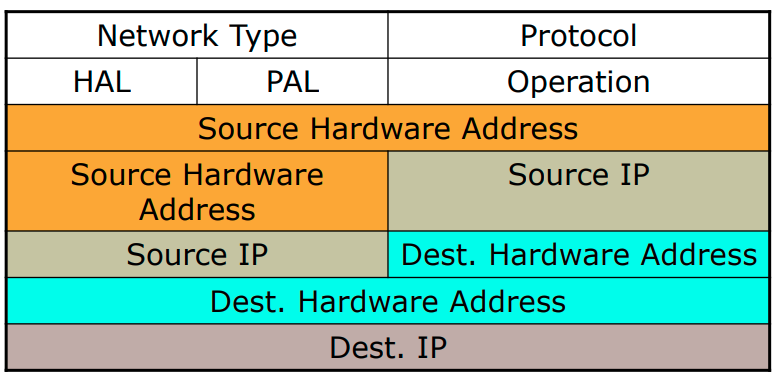
\includegraphics[width=15cm]{images/02/06}
\end{figure}

\begin{itemize}
    \item Network Type~--- тип протокола (для Ethernet~--- 1)
    \item Protocol~--- протокол сетевого уровня (IP~--- 2048)
    \item HAL~--- длина канального адреса (для MAC~--- 6 байт)
    \item PAL~--- длина сетевого адреса (для IP~--- 4 байта)
    \item Operation~--- тип операции (1~--- запрос, 2~--- ответ)
\end{itemize}

Этот протокол абсолютно незащищённый. Нет аутентификации. В открытом виде идёт запрос и в открытом виде идёт ответ. Можно просто обмануть и отправить ответ от своего имени. Хакер должен находиться в той же сети, что и жертва. 

Но при этом и запрашивающий компьютер получит два ответа, и второй узел увидит, что кто-то пытается использовать его адрес.

Поэтому хитрые хакеры на какое-то время выводят узел с запрашиваемым IP из строя.

Вариант защититься~--- всего один. Прописывать адреса ключевых узлов статически.

Эта атака нечастая, потому что хакер должен быть в вашей локальной сети.

А вот в старых виндах была проблема, что даже если вы прописали адрес маршрутизатора статически, то всё равно раз в минуту посылался ARP-запрос. В общем, не сидите в открытой сети с Windows 95.

Протокол ARP, так же как и IP, инкапсулируется прямо в канальный уровень.

\Subsubsection{Групповая доставка}

Раньше мы говорили об индивидуальной доставке. Но что если нам нужна групповая?

Во-первых, тогда нам (маршрутизатору) нужно будет знать о наличии групповых адресов в сегменте, чтобы не забивать канал групповыми сообщениями, если это не надо.

Во-вторых, маршрутизатор должен периодически получать информацию о членстве в группах.

В третьих, нам нужен способ доставки групповых пакетов узлам. То есть нужно соответствие меду групповыми адресами сетевого и канального уровней.

Для индивидуальной адресации этим занимался протокол ARP, а для групповой это делается по-другому. 

В Ethernet адреса вида {\tt 01:xx:xx:xx:xx:xx} зарезервированы под групповые.

Конкретно под TCP/IP зарезервировали диапазон {\tt 01:00:5e:00:00:00-01:00:5e:7f:ff:ff}. Это 23 разряда.

Соостветствие между групповыми Ethernet и IP адреса~--- просто копирование младших 23 разрядов IP адреса в эти 23 разряда канального адреса.

Но в классе D было 28 разрядов, то есть мы игнорируем верхние 5 разрядов. В таком случае коллизии разрешаются уже на приёмной станции (если видим, что этот пакет не к нам~--- выкидываем).

А как маршрутизатор узнает, есть ли в сегменте групповые адреса? Для этого используется протокол {\bf IGMP}.

Весь следующий рассказ про {\bf IGMP v1}.

Он предназначен, чтобы информировать маршрутизатор о том, что в сегменте есть члены какой-то группы.

\begin{enumerate}
    \item Запрос: <<Есть ли подписчики такой-то группы в этом сегменте?>>
    \item Подписчики делают случайную задержу и посылают ответ: <<Да, есть!>>

    Случайная задержка нужна для того, чтобы если у нас есть 100500 подписчиков в сегменте, то один из них (с минимальной задержкой) отошлёт ответ, остальные это увидят и свой ответ посылать не будут (маршрутизатору важно знать, что хоть кто-то там есть).
    \item Если на какой-то запрос не пришёл ответ (через таймаут), то маршрутизатор считает, что подписчиков этой группы нет.
\end{enumerate}

Формат пакета IGMP v1:

\begin{figure}[H]
  \centering
  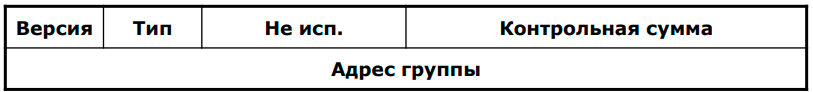
\includegraphics[width=15cm]{images/02/07}
\end{figure}

\begin{itemize}
    \item Тип~--- запрос (1) или ответ (2)
    \item Адрес группы~--- в запросе~--- 0, в ответе~--- номер группы, о которой мы нотифицируем маршрутизатор <<Эта группа есть в данном сегменте>>
\end{itemize}

Протокол IGMP инкапсулируется в протокол IP. В IP-пакете используется:
\begin{itemize}
    \item Адрес {\tt 224.0.0.1}
    \item TTL=1 (чтобы не маршрутизировался)
\end{itemize}

IGMP v2 обратно совместим с v1.

\begin{figure}[H]
  \centering
  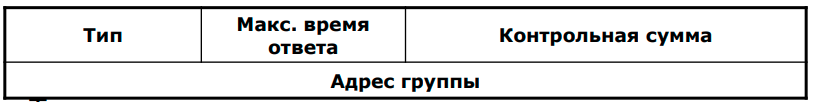
\includegraphics[width=15cm]{images/02/08}
\end{figure}

Поле <<Тип>> занимает 1 байт.
\begin{itemize}
    \item {\tt 0x11}~--- запрос о членстве в группах или конкретной группе
    \item {\tt 0x16}~--- отчёт о членстве v2
    \item {\tt 0x17}~--- нотификация о покидании группы
    \item {\tt 0x12}~--- отчёт о членстве v1 (для совместимости)
\end{itemize}

Максимальное время ответа в 0.1 секунды.

IGMP v3 обратно совместим с v1 и v2.

Позволяет запросить несколько групп и отчитаться о членстве в нескольких группах.

Все версии протокола IGMP не шифруются (а значит, такие же слабости, как и у ARP).

Протокол IP тоже не шифруется, у него нет никаких средств защиты, кроме контрольной суммы, которая тоже такое себе средство защиты. Поэтому вся защита сделана на более высоких уровнях.

\Subsection{Протокол ICMP}

Это протокол сетевого уровня для:
\begin{itemize}
    \item Управления
    \item Нотификации об ошибках и проблемах
    \item Тестирования и мониторинга
\end{itemize}

Инкапсулируется в IP. 

Общая часть пакета:

\begin{figure}[H]
  \centering
  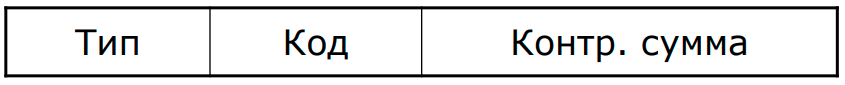
\includegraphics[width=15cm]{images/02/09}
\end{figure}

\begin{itemize}
    \item Тип~--- тип пакета
    \item Код~--- расшифровывает детали внутри типа
    \item Контрольная сумма~--- вычисляется для всего пакета
\end{itemize}

\Subsubsection{Нотификационные сообщения}

\begin{itemize}
    \item Получатель недостижим (3)\\
    \begin{figure}[H]
        \centering
        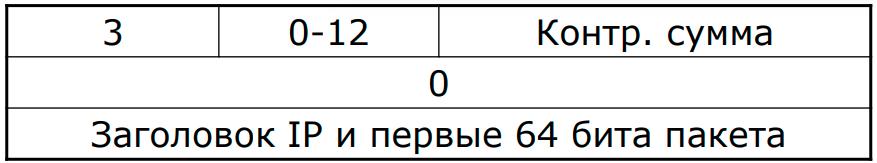
\includegraphics[width=15cm]{images/02/10}
        \end{figure}

    Причины недоступности:
    \begin{itemize}
        \item 0~--- сеть недостижима
        \item 1~--- узел недостижим
        \item 2~--- протокол недостижим
        \item 3~--- порт недостижим
        \item 4~--- требуется фрагментация
        \item 5~--- маршрутизация от источника
        \item 6~--- сеть назначения неизвестна
        \item 7~--- узел назначения неизвестен\\
        6 и 7 чаще всего связаны с использованием невалидных адресов. Например, класса E
        \item 8~--- отправитель изолирован
        \item 9~--- взаимодействие с сетью назначения административно запрещено
        \item 10~--- взаимодействие с узлом назначения административно запрещено\\
        9 и 10 означают, что пакет не был пропущен файерволом
        \item 11~--- сеть недостижима из-за класса обслуживания
        \item 12~--- узел недостижим из-за класса обслуживания
    \end{itemize}
    Такой пакет все файерволы обязаны пропускать
    \item Превышено время (11)\\
    \begin{figure}[H]
        \centering
        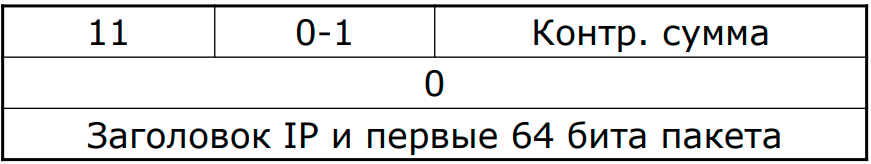
\includegraphics[width=15cm]{images/02/11}
    \end{figure}
    Если код 0, то истёк TTL, иначе превышено время ожидания фрагмента при сборке\\
    Его тоже нельзя фильтровать
    \item Ошибка параметра (12)~--- например, ошибка в контрольной сумме или ошибка при заполнении поля\\
    \begin{figure}[H]
        \centering
        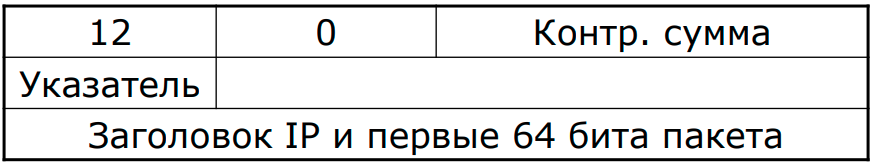
\includegraphics[width=15cm]{images/02/12}
    \end{figure}
    Указатель показывает на номер байта, в котором была обнаружена ошибка\\
    Его тоже нельзя фильтровать на файерволе
\end{itemize}


\Subsubsection{Управляющие сообщения}

\begin{itemize}
    \item Подавление источника (4)\\
    \begin{figure}[H]
        \centering
        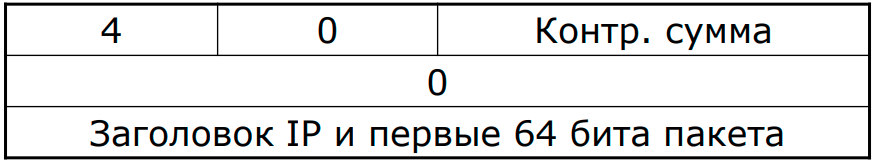
\includegraphics[width=15cm]{images/02/13}
    \end{figure}
    Например, если нам что-то очень интенсивно шлют, мы можем послать сообщение <<СНизь скорость передачи!>>\\
    В реальности почти не используется. ФИльтровать нежелательно
    \item Изменение маршрута\\
    \begin{figure}[H]
        \centering
        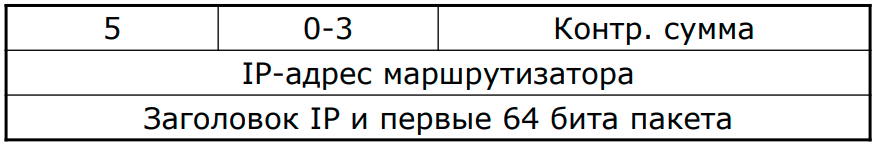
\includegraphics[width=15cm]{images/02/14}
    \end{figure}
    Часто бывает такое, что маршрутизатор понимает, что путь через него неоптимален. Тогда он может отправить это сообщение источнику и сказать: <<Передавать через вот этого товарища оптимальнее, чем через меня!>>\\
    Но при этом мы не можем доверять этому сообщения, ведь оно могло быть от злоумышленника.\\
    Такие пакеты обязательно нужно фильтровать
\end{itemize}

\Subsubsection{Тестовые и контрольные сообщения}

\begin{itemize}
    \item Запрос эха (8) и ответ на запрос эха (0)~--- ping и pong\\
    \begin{figure}[H]
        \centering
        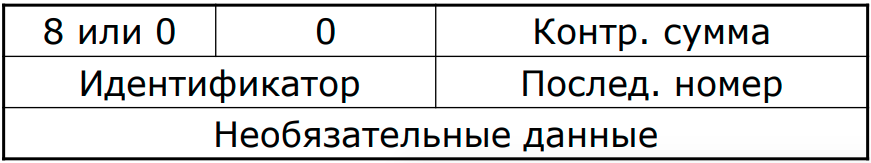
\includegraphics[width=15cm]{images/02/15}
    \end{figure}
    Идентификатор~--- уникальный идентификатор, формирующийся случайным образом, при посылке.\\
    Последовательный номер~--- номер пакета в серии\\
    Необязательные данные сторона-получатель должна повторить в эхо-ответе\\
    Очень часто такие входящие или исходящие пакеты запрещены в корпоративных сетях 
    \item Запрос временной метки (13) и ответ на запрос временной метки (14)\\
    \begin{figure}[H]
        \centering
        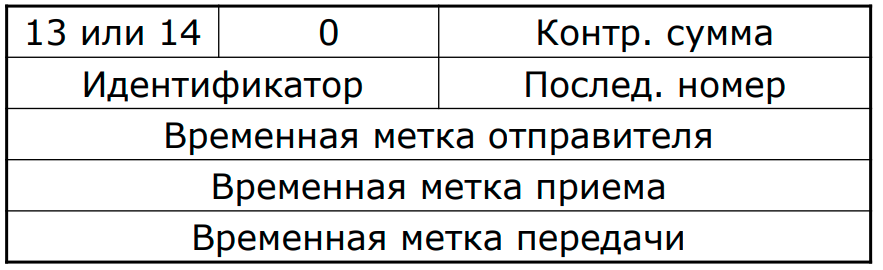
\includegraphics[width=15cm]{images/02/16}
    \end{figure}
    Время в стандартном UNIX-формате. Но с ним нужно быть аккуратным, потому что оно может быть не синхронизированно
    \item Запрос маски адреса (17) и ответ на запрос маски адреса (18)\\
    \begin{figure}[H]
        \centering
        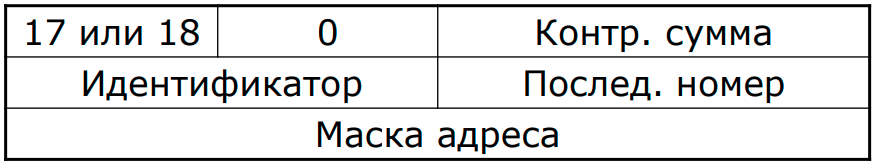
\includegraphics[width=15cm]{images/02/17}
    \end{figure}
    Отвечающий заполняет поле <<Маска адреса>>. Тоже такой себе пакет, потому что позволяет получить информацию о структуре сети. Хакеры строили с его помощью карту сети. Файерволы должны фильтровать.
\end{itemize}